% !TeX spellcheck = en_US
\addscenariosection{1}{Clash Scenario}{The Fractured Kingdoms}{\images/two_way_monolith.png}

\begin{multicols}{2}

\textbf{Author:} mopo

\textit{A terrible Armageddon has struck the lands. Five rulers have found their kingdoms broken and torn apart, but after some time has passed, they discovered their lands had drifted in the magic-laden space of this universe to collide with one another. All five recognize that their first priority must be to rebuild and regrow, and they form a five-kingdom alliance. However, each also knows in the back of their minds that whoever breaks the alliance first, would gain a sharp first-strike advantage...}

\subsection*{\MakeUppercase{Scenario Length}}
This Scenario is played over 16 Rounds.

\subsection*{\MakeUppercase{Player Setup}}
\textbf{Player Count:} 5 free-for-all

\textbf{Starting Resources:} 10 \svg{gold}, 6 \svg{building_materials}, 1 \svg{valuables}

\textbf{Starting Income:} 10 \svg{gold}, 0 \svg{building_materials}, 0 \svg{valuables}

\textbf{Starting Units:}
\begin{itemize}
  \item 3 × A Few \bronze\ Units
\end{itemize}

\textbf{Town Buildings:} \bronze\ Dwelling

\subsection*{\MakeUppercase{Map Setup}}
Take the following Map Tiles and arrange them as shown in the Scenario map layout:

\begin{itemize}
  \item 5 × Starting (I) Map Tile; \textbf{rotate them} so that their \textbf{blocked Fields} match the ones marked in the Scenario map layout
  \item 10 × Near (IV--V) Map Tile
  \item 10 × Far (II--III) Map Tile
  \item 5 × Center (VI--VII) Map Tile
\end{itemize}

\subsection*{\MakeUppercase{Victory Conditions}}
Score the most Victory Points (VPs) by the end of the \nth{16} Round.

\subsection*{\MakeUppercase{Timed Events}}

\textbf{\nth{4} Round:}
\begin{itemize}
  \item All yellow borders on the Starting (I) Map Tiles are ignored until the end of the game.
\end{itemize}
\textbf{\nth{6}, \nth{9} and \nth{12} Rounds:}
\begin{itemize}
  \item Remove all Black Cubes from every Water Wheel and Windmill.
\end{itemize}

\subsection*{\MakeUppercase{Additional Rules}}
Before this Scenario:

\begin{itemize}
  \item Split the Artifact Deck by rarity into 3 separate Decks (Minor, Major, and Relic).
    A player may gain only Minor Artifacts on Starting or Far Tiles, Minor or Major Artifacts on Near Tiles, and Major or Relic Artifacts on Center Tiles.
  \item Split the Spell Deck into 2 separate Decks (Basic and Expert Spells). Magic Arrow is a Basic Spell.
    A player may gain only Basic Spells on Starting or Far Tiles, Expert Spells on Near or Center Tiles.
\end{itemize}

During this Scenario:

\begin{itemize}
  \item Each \svg[12]{movement_token_green} in the map layout is a one-way monolith.
    Any Hero on the Field an \svg[12]{movement_token_green} points away from can pay 1 \svg{movement} to go to the Field that \svg[12]{movement_token_green} is pointing to.
  \item You can defend your Town with your Hero if you have your Main Hero on your Starting (I) Map Tile.
\end{itemize}

Victory Points are counted in accordance to the Tournament book. Additionally, you get:
\begin{itemize}
  \item 2 VP for flagging a Dragon Utopia for the first time
  \item 2 VP for having the Dragon Utopia flagged at the end of the game
  \item 5 VP for bringing the Grail to your Faction Town OR 3 VP for being in possession of the Grail at the end of the game
\end{itemize}

\subsection*{\MakeUppercase{Optional Rules}}
\begin{itemize}
  \item All \svg[12]{movement_token_green} indicate two-way monoliths instead of one-way.
    Heroes can travel in either direction by paying 1~\svg{movement}.
  \item The monoliths start inactive (place them the inactive \svg[12]{movement_token_red} side up).
    Heroes must pay 1~\svg{building_materials} and 1~\svg{movement} to activate them.
  \item Heroes can destroy monoliths by paying 1~\svg{movement}.
    Flip a destroyed monolith to the \svg[12]{movement_token_red} side up.
\end{itemize}

\end{multicols}

\vspace*{-8em}

\begin{tikzpicture}[overlay, remember picture]

  \newcommand{\blocked}[3]{%
    % Parameters: #1 = x-coordinate, #2 = y-coordinate, #3 = rotation angle
    \begin{scope}[shift={(#1,#2)}, rotate=#3]
      \iftoggle{noartbackground}
      {\draw[draw=darkyellow, thick, pattern=north east lines, pattern color=darkyellow]}
      {\draw[draw=yellow!40!white!90!brown, line width=1.4pt, draw opacity=0.9, fill=yellow!50!white!80!brown, fill opacity=\iftoggle{noartbackground}{0.9}{0.5}]}
        (0:0.56cm) -- (60:0.56cm) -- (120:0.56cm) --
        (180:0.56cm) -- (240:0.56cm) -- (300:0.56cm) -- cycle;
    \end{scope}
  }

  \newcommand{\arrow}[3]{
    % Parameters: #1 = x-coordinate, #2 = y-coordinate, #3 = rotation angle
    \node[rotate=#3, opacity=0.5] at ([shift={(2pt,-2pt)}]#1,#2) {
\includegraphics[height=23px]{\images/movement_token_shadow.png}};
    \node[rotate=#3] at (#1, #2) {\svg[20]{movement_token_green}};
  }

  \node(bg)[anchor=center, opacity=0.07, xshift=2em, yshift=-9.5em] at (current page.center) {
    
\includegraphics[width=1.2\paperwidth, keepaspectratio]{\art/two_way_monolith.png}
  };

  \node at (9, -12) {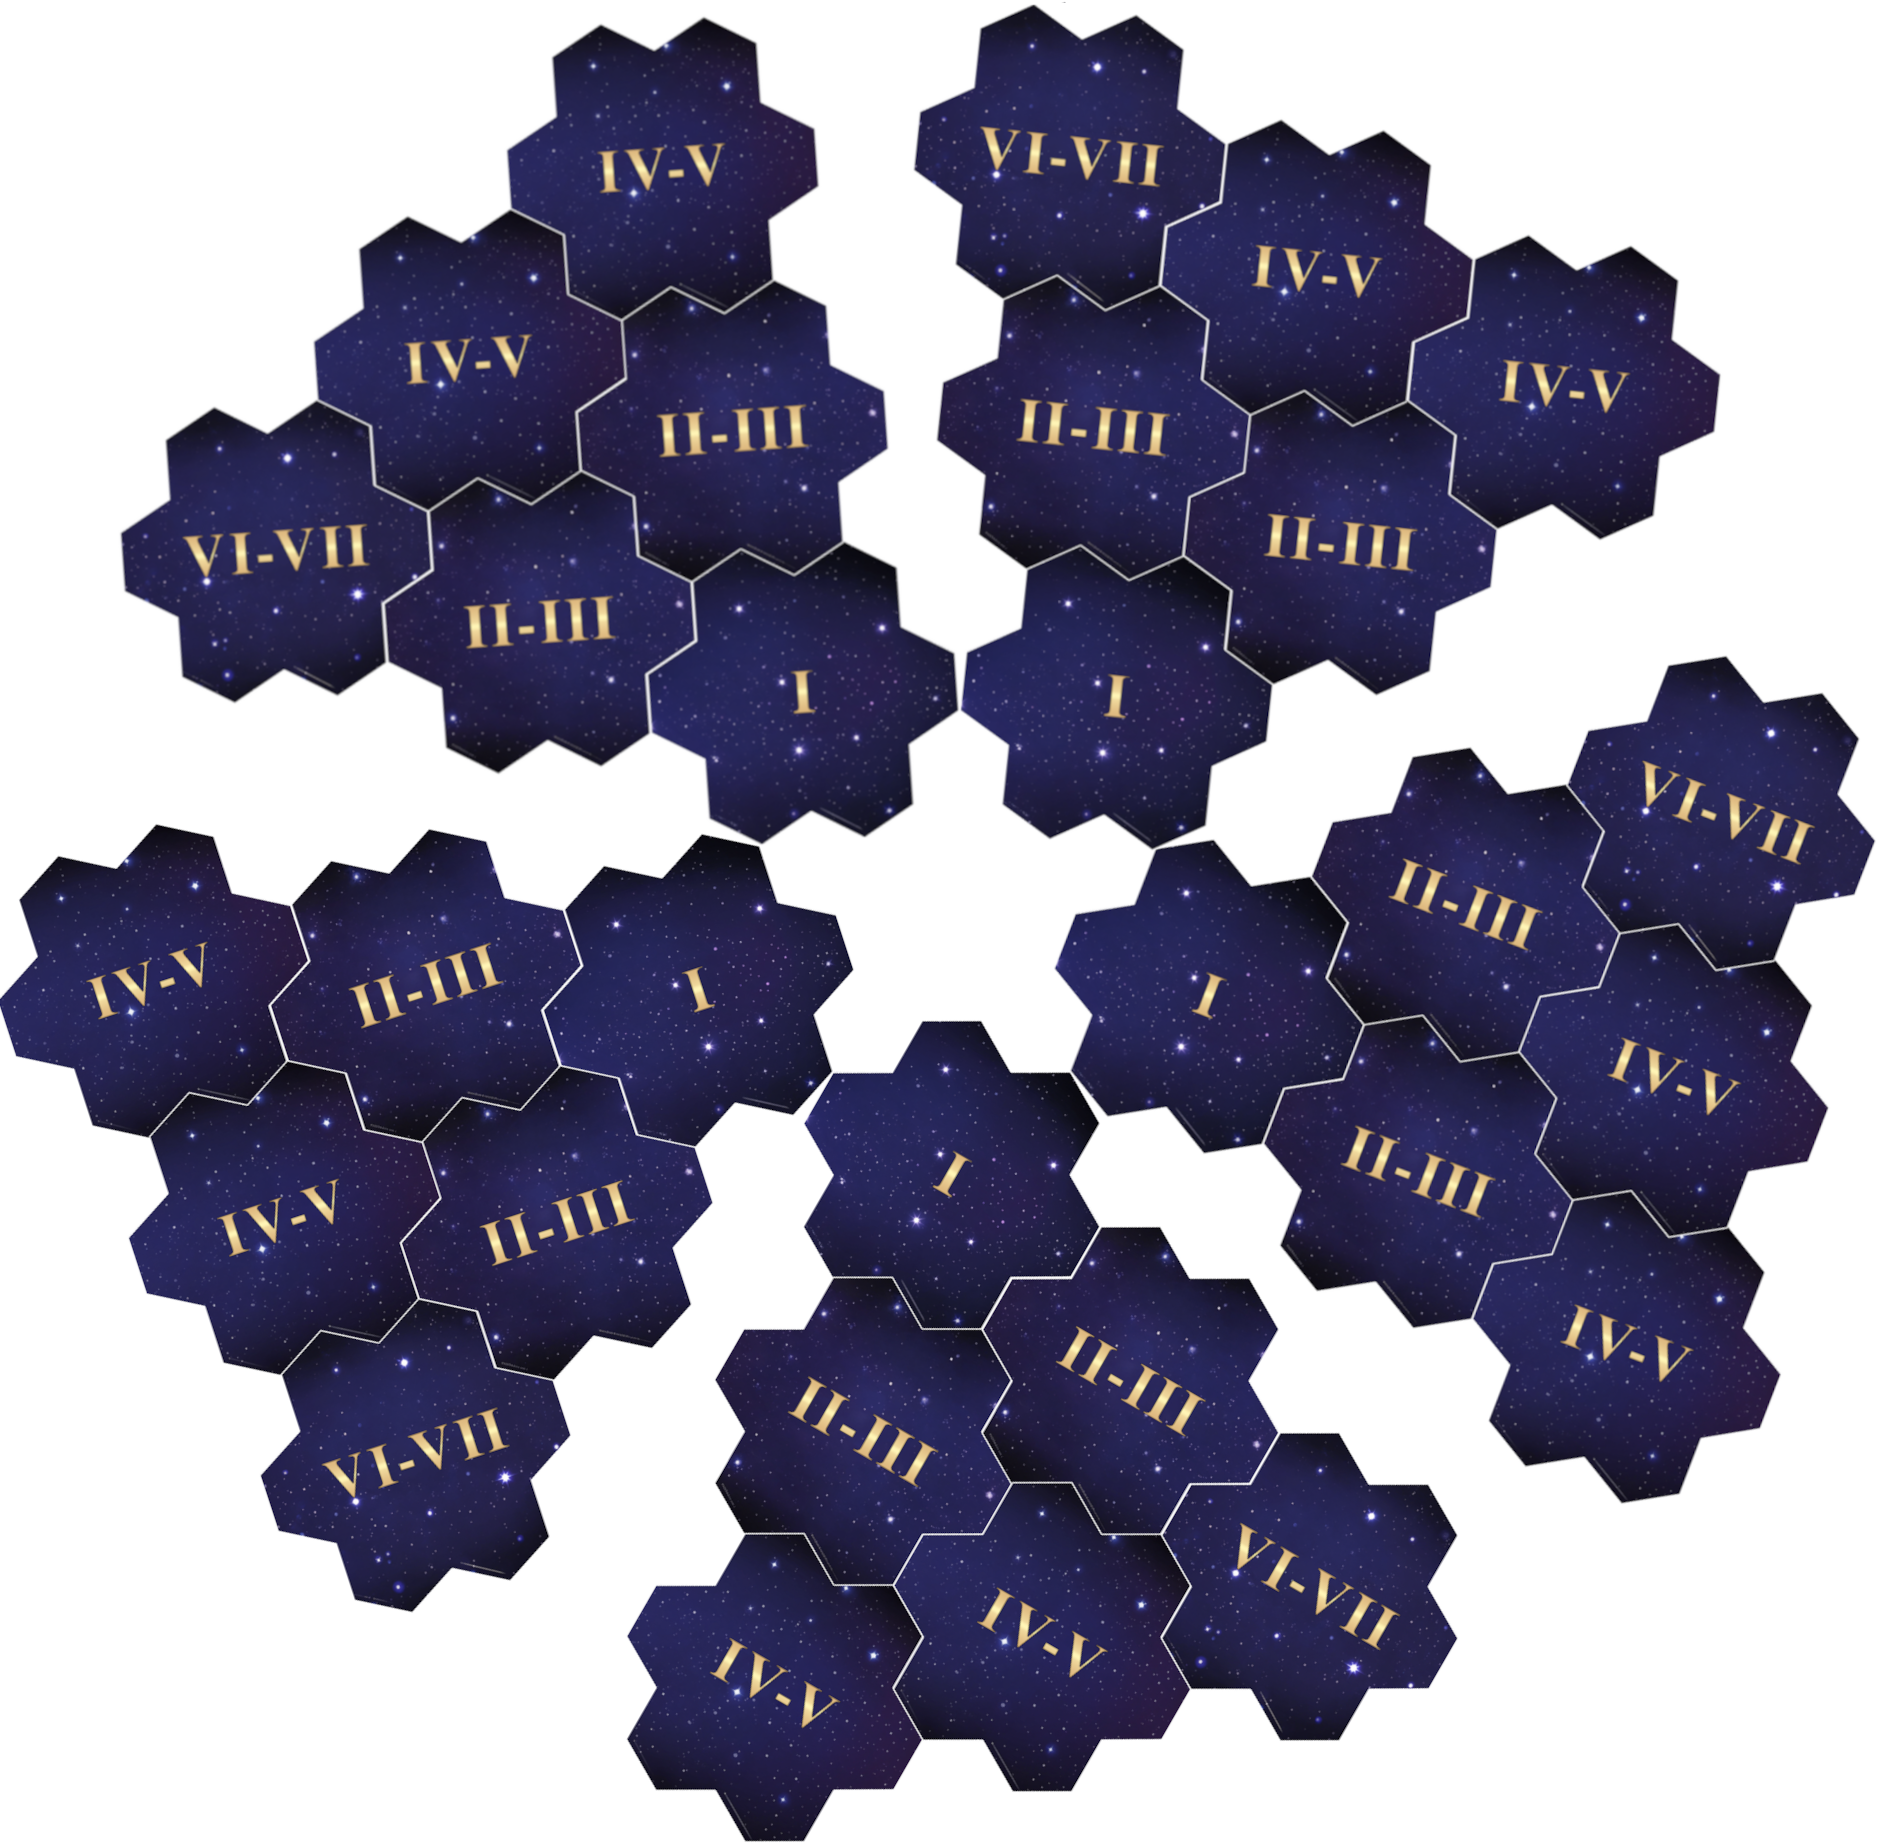
\includegraphics[width=0.9\paperwidth]{\maps/the_fractured_kingdoms.png}};

  \arrow{12.35}{-15.7}{-142}
  \arrow{14.4}{-17.6}{38}

  \arrow{13.91}{-9.95}{-72}
  \arrow{16.2}{-8.55}{108}

  \arrow{8.2}{-4.35}{-176}
  \arrow{8.75}{-6.9}{4}

  \arrow{1.5}{-10.35}{-99}
  \arrow{4.2}{-10.75}{81}

  \arrow{6.65}{-16.1}{155}
  \arrow{5.45}{-18.7}{-25}

  \blocked{7.05}{-8.85}{-25.5}

  \blocked{11.40}{-8.87}{23}

  \blocked{12.69}{-13.12}{67.7}

  \blocked{9.135}{-15.58}{0}

  \blocked{5.58}{-13.01}{-71}


\end{tikzpicture}
